\documentclass[11pt]{article}
\usepackage{geometry}
\geometry{letterpaper, margin=1in}
\usepackage[utf8]{inputenc}
\usepackage{graphicx}
\usepackage{upgreek}
\usepackage{hyperref}
\usepackage[T1]{fontenc}
\usepackage{amsmath}
\usepackage[colorinlistoftodos]{todonotes}
\usepackage{float}
\usepackage{minted} 

\title{ECE532S Digital Systems Design \\ \vspace{0.4cm}
       \Large Tutorial 5 - TCP Client on Microblaze Using LWIP \\ \vspace{0.4cm}
       \small Last Updated: July, 2019}
\author{ }
\date{ }

\begin{document}
\maketitle
\vspace{-1cm}

The goal of this tutorial is to demonstrate how to implement an LWIP-based TCP client on the Nexsys DDR board. LWIP is a specific low-overhead implementation of the TCP/IP stack that Xilinx has implemented for their MicroBlaze processor. The LWIP client introduced in this tutorial will be implemented using the Xilinx SDK, running on a Microblaze-based SoC system. This tutorial builds upon other tutorials already presented earlier in the course. The tutorial will demonstrate how to setup an LWIP connection as a client, how to setup the callback functions to respond to ACKs and received packets, and how to connect to a TCP echo server on a host computer to the test the functionality of the LWIP client.

\section*{Step 1 - Digilent LWIP Server Tutorial}
The LWIP client presented in this tutorial is based on the system and software environment setup in the Digilent LWIP echo server tutorial. Therefore, as a first step, you are required to go through and implement the described systems of that tutorial. For the Nexsys DDR board, the tutorial is available \href{https://reference.digilentinc.com/learn/programmable-logic/tutorials/nexys-4-ddr-getting-started-with-microblaze-servers/start}{\color{blue}here}. Some changes must be made to the tutorial for our purposes, so please follow the tutorial based on the steps and required modifications listed below.

\begin{enumerate}
    \item Create a new project according to Step 1
    \item Create a new Block Design with a Microblaze system according to Step 2
    \begin{enumerate}
        \item Perform steps 2.1 through 2.4
        \item Before step 2.5, double click on the Microblaze core in order to customize it
        \item Go to page 4 of the customization window, as depicted in Figure~\ref{fig:mb_cust4}
        \item Select to \textit{Enable Peripheral AXI Instruction Interface}, and click OK
        \begin{itemize}
            \item This will allow the Microblaze to fetch instructions from peripherals connected to the AXI bus, which is required since an LWIP application is often too big to fit into available BRAM resources and thus we need to use the DDR memory
        \end{itemize}
        \item Proceed with steps 2.5 through 2.10
    \end{enumerate}
    \item Follow steps 3 through 11 according to the tutorial
    \begin{itemize}
        \item We will be using the LWIP echo server example application selected in Step 8 as the template for our LWIP TCP client implementation
    \end{itemize}
    \item Optionally, run though steps 12 to 14 to test the LWIP echo server application (this may be a useful exercise if you want to implement an LWIP server application in the future)
    \begin{itemize}
        \item Step 12 differs from our previous tutorials due to different versions of Vivado. Use the steps from our previous tutorials in order to create a \textit{Run Configuration} and connect to the \textit{SDK Terminal}.
    \end{itemize}
\end{enumerate}

\begin{figure}[t]
\centering
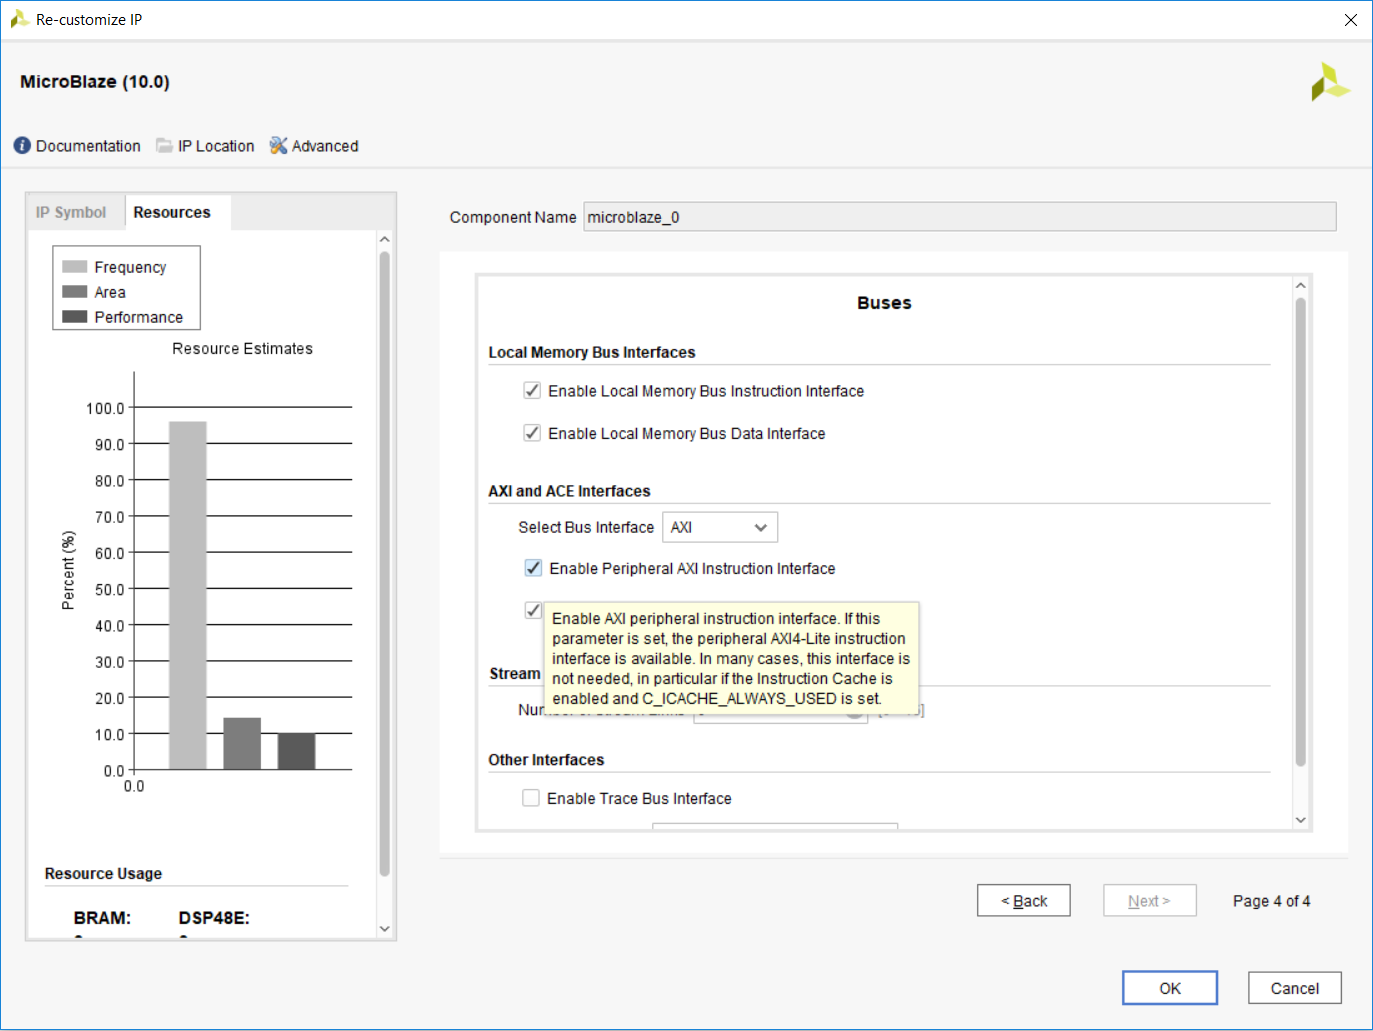
\includegraphics[width=\textwidth]{mb_cust4.png}
\caption{Microbalze customization interface (page 4) showing how to enable the Peripheral AXI Interface for instructions}
\label{fig:mb_cust4}
\end{figure}

\section*{Step 2 - Modifications to Create LWIP Client}
The SDK project, as created according to the LWIP echo server example project, can be modified into an LWIP cleint application instead. In this section, we describe how to create a simple LWIP TCP client that simply sends a single packet once a connection to a TCP server has been established. The TCP server will be implemented on an x86 host using an included python script.

\begin{enumerate}
    \item Replace the \textit{main.c} file of the echo server application with the \textit{main.c} file packaged with this tutorial
    \item Delete the \textit{echo.c} file from the application, since it will no longer be needed
    \item Connect the Nexsys DDR board to your host x86 machine using an Ethernet cable
    \item Setup the network connection on your host x86 machine according to steps 14.1 through 14.2.5 of the Digilent tutorial
    \begin{itemize}
        \item These instructions are based on a Windows 7 operating system, please find the correct steps for your particular system
    \end{itemize}
    \item Make sure to turn off the firewall on your host machine
    \item Run the \textit{echo.py} Python script packaged with this tutorial, this will start a TCP echo server on your host machine on Port 22, see Figure~\ref{fig:echo_py}
    \item Back in the Vivado SDK environment, connect to the \textit{SDK Terminal} according to the steps outlined in previous tutorials (e.g. baud rate of 9600)
    \item Run the LWIP client application according to step 12 of the Digilent tutorial
    \begin{itemize}
        \item Step 12 differs from our previous tutorials due to different versions of Vivado. Use the steps from our previous tutorials in order to create and run a \textit{Run Configuration}.
    \end{itemize}
    \item Verify that the packet was received by the x86 echo server (the packet data should have printed to the python terminal), and that the echoed packet was received by the LWIP client on the FPGA (the packet data should have printed to the SDK terminal)
\end{enumerate}

\begin{figure}[t]
\centering
\begin{minted}
[
frame=lines,
framesep=2mm,
baselinestretch=1.2,
bgcolor=white,
fontsize=\footnotesize,
]
{python}
import socket

def listen():
    connection = socket.socket(socket.AF_INET, socket.SOCK_STREAM)
    connection.setsockopt(socket.SOL_SOCKET, socket.SO_REUSEADDR, 1)
    connection.bind(('0.0.0.0', 22))
    connection.listen(10)
    print("Server opened on port 22")
    while True:
        current_connection, address = connection.accept()
        while True:
            data = current_connection.recv(2048)

            if data == 'quit\r\n':
                current_connection.shutdown(1)
                current_connection.close()
                break

            elif data == 'stop\r\n':
                current_connection.shutdown(1)
                current_connection.close()
                exit()

            elif data:
                current_connection.send(data)
                print (data)


if __name__ == "__main__":
    try:
        listen()
    except KeyboardInterrupt:
        pass
\end{minted}
\vspace{-0.7cm}
\caption{Python script to run an echo server on port 22}
\label{fig:echo_py}
\end{figure}

\section*{Understanding the LWIP Client Code}
The LWIP client code may seem daunting to understand, but the structure of LWIP and its callbacks is actually relatively straightforward. To familiarize yourself generally with the structure of LWIP calls and callbacks, see the LWIP Wiki page for the \href{http://lwip.wikia.com/wiki/Raw/TCP}{\color{blue}RAW API}. An especially useful part of the Wiki is the \textit{Raw TCP Sample Sequence Diagrams} section, which diagrams the sequence of calls necessary for using LWIP. Note, LWIP is implemented in an abstracted way with many layers of available calls. We use the lowest layer, the RAW layer, since we are running without an OS and thus do not have access to threading functionality.

In this section, we will outline the contents of the \textit{main.c} file in order to ease the learning curve for the LWIP API. To ease readability, the main function and all of the LWIP setup and callback functions are included in this one file, but you may wish to split it into separate files for modularity.

\subsubsection*{Preprocessor Directives and Global Variables}
The first part of the code is shown in Figure~\ref{fig:code_pre}. Here we include all of the files that are required for our LWIP client implementation. There's nothing too special about this code, though note the \textit{void lwip\_init();} function prototype included. This is required since this declaration is missing from the header files of the Xilinx LWIP implementation. After the includes, macros are defined for the network parameters of the device. The IP parameters are defined as strings (with the later \textit{inet\_aton} function converting it to the required format), while the MAC parameters are defined as char arrays and the port numbers as integers. The project also includes a macro for the size of the packet to send.

Next, Figure~\ref{fig:code_glovar} shows the global variables included in the project. The first global variable is required if we have DHCP enabled. This variable is modified elsewhere in the project and is simply referenced in this code to detect a DHCP timeout. In our test setup, we didn't have a DHCP server, and thus the timeout was always reached. In any case, include this if DHCP is to be used. Next, two additional \textit{extern} timer variables are used to determine when it is necessary to run the TCP control functions (these must always be included), and then global variables which store the current network interface handler, the protocol control block (PCB) handler, and a simple variable that indicates when a connection has been established are included.

\subsubsection*{Main Function}

At the beginning of the main function, we setup our network interface connection. This is shown in the code fragment in Figure~\ref{fig:code_main_net}. The code here declares variables to store the IP network parameters, initializes the LWIP environment, and then calls the Xilinx function \textit{xemac\_add(...)} to add the Network interface of our project to the network interfaces list. Once that has been done, the interupts are enabled and LWIP is notified that the network is up.

After setting up the network interface, the DHCP protocol is implemented in a loop until either an IP address is assigned or a timeout is reached. This is shown in Figure~\ref{fig:code_main_dhcp}. The \textit{dhcp\_start} function starts the DHCP process. Inside the loop that waits for the end of the DHCP process, the function \textit{xemacif\_imput(...)} is called. This function is called to take all of the data that has been received since its last invocation and pass that data to LWIP to be processed. This data is orignially buffered by the interrupt handler for the Ethernet controller, but it is not seen by LWIP until we call this function. If DHCP fails, we assign default values using our preprocessor macros.

Finally, we get to the main part of the application, shown in Figure~\ref{fig:code_main}. Before the main event loop, we have a call to a function we've created to setup the TCP connection and connect to the remote server. Then, inside the event loop, we first check our \textit{extern} TCP variables to determine whether LWIP needs to do some TCP processing. This check must be done periodically (on the order of 250 milliseconds) for LWIP to function correctly. Then, we call our \textit{xemacif\_input(...)} function to handoff any new data received to LWIP to be processed. Finally, at the end of the event loop, any additional code that needs to be run periodically can be added. Any code added here should be non-blocking (i.e. so that the TCP processing part of the loop can be checked regularly). Note also that the \textit{is\_connected} global variable we've declared can be used here if any of the functionality depends on whether or not a TCP connection has been established.

\subsubsection*{Setting Up the TCP Client Connection}
The TCP client connection is created in the \textit{setup\_client\_connection()} function defined underneath the main function, see Figure~\ref{fig:code_setup_conn}. The first thing to note in this function is the new TCP protocol control block (PCB) created with the function \textit{tcp\_new\_ip\_type(...)}. This function call is required to start the TCP connection creation process. Next, the call to function \textit{tcp\_bind(...)} binds the connection to a certain source port (Note, the \textit{tcp\_bind(...)} call is optional for client TCP projects). Finally, the function \textit{tcp\_connect(...)} initiates the client connection to the server. As parameters, the \textit{tcp\_connect(...)} function accepts the remote IP address to connect to, the destination port to connect to, and a callback function to be executed when the connection is made.

\subsubsection*{TCP Connection Completed Callback}
Once a connection has been established with the server, the callback function associated with the \textit{tcp\_connect(...)} instance that initiated that connection will be called. The function we've used in our implementation is shown in Figure~\ref{fig:code_conn_callback}. First we check for an error in establishing the connection, and close the client connection if we do have an error. Otherwise, we make sure to store the new protocol control block handler (PCB) handler in the global variable we've created so other functions can access the TCP connection.

The next step is to set the callback functions for various aspects of the the TCP connection (Note, these callbacks can also be setup in the previous function). The \textit{tcp\_arg(...)} function specifies the arguments to be used for all of the callbacks. In this case, we don't have any arguments in our callback functions so we leave it as NULL. Next, the three functions \textit{tcp\_recv(...)}, \textit{tcp\_sent(...)}, and \textit{tcp\_err(...)} are used to set the callback functions to be used when new data has been received, when a sent packet has been ACKed, and when an error is encountered respectively.

Once the callback functions have been established, we can add our own code to enable whatever functionality we're hoping to implement. In our case, we'd like to send a single packet once the connection is established. To send a packet, two different functions are used. First, \textit{tcp\_write(...)} is used to enqueue data to be sent; LWIP will not immediately send this data but instead buffer it with the data from future calls to \textit{tcp\_write(...)}. Next, a call to \textit{tcp\_output(...)} will instruct LWIP to take all the buffered data and send it in one or more packets (LWIP determines how to partition the data). See the LWIP wiki for details pertaining to how to set the \textit{apiflags} for calls to \textit{tcp\_write(...)}.

\subsubsection*{Packet Received Callback}
Once a packet is received by LWIP, the callback function we'd indicated is called. The implementation of the callback function in our particular case is shown in Figure~\ref{fig:code_recv_callback}. The packet data is passed as a pointer of \textit{struct pbuf} type, see the \href{http://www.nongnu.org/lwip/2_0_x/group__pbuf.html}{\color{blue}LWIP Packet Buffer Documentation} for information on how the packet data is stored in this data type. If the Packet Buffer pointer is NULL, this indicates that the connection has been closed. Otherwise, we're free to insert our own code to process the packet data. Once the packet data is processed, we must make sure to indicate to LWIP that we've processed the bytes, with a call to \textit{tcp\_recved(tpcb,p->tot\_len)}, so that LWIP knows it can send us more data (or so it can throttle data packet reception if we're too slow). Also, we must make sure to free the Packet Buffer type with a call to \textit{pbuf\_free(p)}.

In our client implementation, we simply read the packet data and print it to the SDK Terminal. The implemented code shows an easy (though inefficient) way to access the packet data. The LWIP function \textit{pbuf\_copy\_partial(...)} takes the Packet Buffer pointer, a pointer to a buffer in memory, the length to copy from the packet, and the offset to start the copy. In our case, we indicate the total length of the packet and an offset of zero to copy the whole packet; the packet data is then copied to our buffer. This is of course inefficient because it necessitates a copy action where we could otherwise look at the packet data in place.

\subsubsection*{Packet Send Acknowledgment Callback}
When we send a packet over TCP, the server will send back an ACK signal when it has successfully received that packet. When the ACK is received by LWIP, it calls our indicated \textit{sent} callback function, with our implementation shown in Figure~\ref{fig:code_sent_callback}. We don't necessarily have to do anything in this function (and in fact many LWIP client implementations leave this function blank), but we have a simple print statement to demonstrate the functionality.

\subsubsection*{TCP Error Callback}
When some error is encountered, the callback function we indicated to be called in case of an error is invoked. In our application, this function is shown in Figure~\ref{fig:code_err_callback}. Here we simply close the connection and print that the connection was aborted. To close the connection, we call another function we've created called \textit{tcp\_client\_close(...)}, shown in Figure~\ref{fig:code_close}. In this function we reset all of the callbacks to NULL, and call \textit{tcp\_close(...)} to close the TCP connection.

\begin{figure}[ht]
\centering
\begin{minted}
[
frame=lines,
framesep=2mm,
baselinestretch=1.2,
bgcolor=white,
fontsize=\footnotesize,
]
{c}
//Standard library includes
#include <stdio.h>
#include <string.h>

//BSP includes for peripherals
#include "xparameters.h"
#include "netif/xadapter.h"

#include "platform.h"
#include "platform_config.h"
#if defined (__arm__) || defined(__aarch64__)
#include "xil_printf.h"
#endif
#include "xil_cache.h"

//LWIP include files
#include "lwip/ip_addr.h"
#include "lwip/tcp.h"
#include "lwip/err.h"
#include "lwip/tcp.h"
#include "lwip/inet.h"
#if LWIP_IPV6==1
#include "lwip/ip.h"
#else
#if LWIP_DHCP==1
#include "lwip/dhcp.h"
#endif
#endif

void lwip_init(); /* missing declaration in lwIP */

//TCP Network Params
#define SRC_MAC_ADDR {0x00, 0x0a, 0x35, 0x00, 0x01, 0x02}
#define SRC_IP4_ADDR "192.168.1.10"
#define IP4_NETMASK "255.255.255.0"
#define IP4_GATEWAY "192.168.1.1"
#define SRC_PORT 7

#define DEST_IP4_ADDR  "192.168.1.11"
#define DEST_IP6_ADDR "fe80::6600:6aff:fe71:fde6"
#define DEST_PORT 22

#define TCP_SEND_BUFSIZE 20
\end{minted}
\vspace{-0.7cm}
\caption{Preprocessor Directives of main.c}
\label{fig:code_pre}
\end{figure}

\begin{figure}[ht]
\centering
\begin{minted}
[
frame=lines,
framesep=2mm,
baselinestretch=1.2,
bgcolor=white,
fontsize=\footnotesize,
]
{c}
//DHCP global variables
#if LWIP_IPV6==0
#if LWIP_DHCP==1
extern volatile int dhcp_timoutcntr;
err_t dhcp_start(struct netif *netif);
#endif
#endif

//Networking global variables
extern volatile int TcpFastTmrFlag;
extern volatile int TcpSlowTmrFlag;
static struct netif server_netif;
struct netif *app_netif;
static struct tcp_pcb *c_pcb;
char is_connected;
\end{minted}
\vspace{-0.7cm}
\caption{Global Variables of main.c}
\label{fig:code_glovar}
\end{figure}

\begin{figure}[ht]
\centering
\begin{minted}
[
frame=lines,
framesep=2mm,
baselinestretch=1.1,
bgcolor=white,
fontsize=\footnotesize,
]
{c}
	//Varibales for IP parameters
#if LWIP_IPV6==0
	ip_addr_t ipaddr, netmask, gw;
#endif

	//The mac address of the board. this should be unique per board
	unsigned char mac_ethernet_address[] = SRC_MAC_ADDR;

	//Network interface
	app_netif = &server_netif;

	//Initialize platform
	init_platform();

	//Defualt IP parameter values
#if LWIP_IPV6==0
#if LWIP_DHCP==1
        ipaddr.addr = 0;
	gw.addr = 0;
	netmask.addr = 0;
#else
	(void)inet_aton(SRC_IP4_ADDR, &ipaddr);
	(void)inet_aton(IP4_NETMASK, &netmask);
	(void)inet_aton(IP4_GATEWAY, &gw);
#endif	
#endif

	//LWIP initialization
	lwip_init();

	//Setup Network interface and add to netif_list
#if (LWIP_IPV6 == 0)
	if (!xemac_add(app_netif, &ipaddr, &netmask,
						&gw, mac_ethernet_address,
						PLATFORM_EMAC_BASEADDR)) {
		xil_printf("Error adding N/W interface\n");
		return -1;
	}
#else
	if (!xemac_add(app_netif, NULL, NULL, NULL, mac_ethernet_address,
						PLATFORM_EMAC_BASEADDR)) {
		xil_printf("Error adding N/W interface\n");
		return -1;
	}
	app_netif->ip6_autoconfig_enabled = 1;

	netif_create_ip6_linklocal_address(app_netif, 1);
	netif_ip6_addr_set_state(app_netif, 0, IP6_ADDR_VALID);

#endif
	netif_set_default(app_netif);

	//Now enable interrupts
	platform_enable_interrupts();

	//Specify that the network is up
	netif_set_up(app_netif);
\end{minted}
\vspace{-0.7cm}
\caption{Network interface setup in main function of main.c}
\label{fig:code_main_net}
\end{figure}

\begin{figure}[ht]
\centering
\begin{minted}
[
frame=lines,
framesep=2mm,
baselinestretch=1.2,
bgcolor=white,
fontsize=\footnotesize,
]
{c}
#if (LWIP_IPV6 == 0)
#if (LWIP_DHCP==1)
	/* Create a new DHCP client for this interface.
	 * Note: you must call dhcp_fine_tmr() and dhcp_coarse_tmr() at
	 * the predefined regular intervals after starting the client.
	 */
	dhcp_start(app_netif);
	dhcp_timoutcntr = 24;

	while(((app_netif->ip_addr.addr) == 0) && (dhcp_timoutcntr > 0))
		xemacif_input(app_netif);

	if (dhcp_timoutcntr <= 0) {
		if ((app_netif->ip_addr.addr) == 0) {
			xil_printf("DHCP Timeout\n");
			xil_printf("Configuring default IP of %s\n", SRC_IP4_ADDR);
			(void)inet_aton(SRC_IP4_ADDR, &(app_netif->ip_addr));
			(void)inet_aton(IP4_NETMASK, &(app_netif->netmask));
			(void)inet_aton(IP4_GATEWAY, &(app_netif->gw));
		}
	}

	ipaddr.addr = app_netif->ip_addr.addr;
	gw.addr = app_netif->gw.addr;
	netmask.addr = app_netif->netmask.addr;
#endif
#endif
\end{minted}
\vspace{-0.7cm}
\caption{DHCP loop in main function of main.c}
\label{fig:code_main_dhcp}
\end{figure}

\begin{figure}[ht]
\centering
\begin{minted}
[
frame=lines,
framesep=2mm,
baselinestretch=1.2,
bgcolor=white,
fontsize=\footnotesize,
]
{c}
        //Setup connection
	setup_client_conn();

	//Event loop
	while (1) {
		//Call tcp_tmr functions
		//Must be called regularly
		if (TcpFastTmrFlag) {
			tcp_fasttmr();
			TcpFastTmrFlag = 0;
		}
		if (TcpSlowTmrFlag) {
			tcp_slowtmr();
			TcpSlowTmrFlag = 0;
		}

		//Process data queued after interupt
		xemacif_input(app_netif);



		//ADD CODE HERE to be repeated constantly 
		// Note - should be non-blocking
		// Note - can check is_connected global var to see if connection open
		

		//END OF ADDED CODE


	}
\end{minted}
\vspace{-0.7cm}
\caption{Event loop in main function of main.c}
\label{fig:code_main}
\end{figure}

\begin{figure}[ht]
\centering
\begin{minted}
[
frame=lines,
framesep=2mm,
baselinestretch=1.2,
bgcolor=white,
fontsize=\footnotesize,
]
{c}
int setup_client_conn()
{
	struct tcp_pcb *pcb;
	err_t err;
	ip_addr_t remote_addr;

	xil_printf("Setting up client connection\n");

#if LWIP_IPV6==1
	remote_addr.type = IPADDR_TYPE_V6;
	err = inet6_aton(DEST_IP6_ADDR, &remote_addr);
#else
	err = inet_aton(DEST_IP4_ADDR, &remote_addr);
#endif

	if (!err) {
		xil_printf("Invalid Server IP address: %d\n", err);
		return -1;
	}

	//Create new TCP PCB structure
	pcb = tcp_new_ip_type(IPADDR_TYPE_ANY);
	if (!pcb) {
		xil_printf("Error creating PCB. Out of Memory\n");
		return -1;
	}

	//Bind to specified @port
	err = tcp_bind(pcb, IP_ANY_TYPE, SRC_PORT);
	if (err != ERR_OK) {
		xil_printf("Unable to bind to port %d: err = %d\n", SRC_PORT, err);
		return -2;
	}

	//Connect to remote server (with callback on connection established)
	err = tcp_connect(pcb, &remote_addr, DEST_PORT, tcp_client_connected);
	if (err) {
		xil_printf("Error on tcp_connect: %d\n", err);
		tcp_client_close(pcb);
		return -1;
	}

	is_connected = 0;

	xil_printf("Waiting for server to accept connection\n");

	return 0;
}
\end{minted}
\vspace{-0.7cm}
\caption{Function to setup the TCP client connection, in main.c}
\label{fig:code_setup_conn}
\end{figure}

\begin{figure}[ht]
\centering
\begin{minted}
[
frame=lines,
framesep=2mm,
baselinestretch=1.05,
bgcolor=white,
fontsize=\footnotesize,
]
{c}
static err_t tcp_client_connected(void *arg, struct tcp_pcb *tpcb, err_t err)
{
	if (err != ERR_OK) {
		tcp_client_close(tpcb);
		xil_printf("Connection error\n");
		return err;
	}

	xil_printf("Connection to server established\n");

	//Store state (for callbacks)
	c_pcb = tpcb;
	is_connected = 1;

	//Set callback values & functions
	tcp_arg(c_pcb, NULL);
	tcp_recv(c_pcb, tcp_client_recv);
	tcp_sent(c_pcb, tcp_client_sent);
	tcp_err(c_pcb, tcp_client_err);



	//ADD CODE HERE to do when connection established

	//Just send a single packet
	u8_t apiflags = TCP_WRITE_FLAG_COPY | TCP_WRITE_FLAG_MORE;
	char send_buf[TCP_SEND_BUFSIZE];
	u32_t i;

	for(i = 0; i < TCP_SEND_BUFSIZE-1; i = i + 1)
	{
		send_buf[i] = i+'a';
	}
	send_buf[TCP_SEND_BUFSIZE-1] = '\n';

	//Loop until enough room in buffer (should be right away)
	while (tcp_sndbuf(c_pcb) < TCP_SEND_BUFSIZE);

	//Enqueue some data to send
	err = tcp_write(c_pcb, send_buf, TCP_SEND_BUFSIZE, apiflags);
	if (err != ERR_OK) {
		xil_printf("TCP client: Error on tcp_write: %d\n", err);
		return err;
	}

	//send the data packet
	err = tcp_output(c_pcb);
	if (err != ERR_OK) {
		xil_printf("TCP client: Error on tcp_output: %d\n",err);
		return err;
	}

	xil_printf("Packet data sent\n");

	//END OF ADDED CODE



	return ERR_OK;
}
\end{minted}
\vspace{-0.7cm}
\caption{Callback function called once connection established, in main.c}
\label{fig:code_conn_callback}
\end{figure}

\begin{figure}[ht]
\centering
\begin{minted}
[
frame=lines,
framesep=2mm,
baselinestretch=1.2,
bgcolor=white,
fontsize=\footnotesize,
]
{c}
static err_t tcp_client_recv(void *arg, struct tcp_pcb *tpcb, struct pbuf *p, err_t err)
{
	//If no data, connection closed
	if (!p) {
		xil_printf("No data received\n");
		tcp_client_close(tpcb);
		return ERR_OK;
	}



	//ADD CODE HERE to do on packet reception

	//Print message
	xil_printf("Packet received, %d bytes\n", p->tot_len);

	//Print packet contents to terminal
	char* packet_data = (char*) malloc(p->tot_len);
	pbuf_copy_partial(p, packet_data, p->tot_len, 0); //Note - inefficient way to access packet data
	u32_t i;

	for(i = 0; i < p->tot_len; i = i + 1)
		putchar(packet_data[i]);

	//END OF ADDED CODE



	//Indicate done processing
	tcp_recved(tpcb, p->tot_len);

	//Free the received pbuf
	pbuf_free(p);

	return 0;
}
\end{minted}
\vspace{-0.7cm}
\caption{Callback function called when packet received, in main.c}
\label{fig:code_recv_callback}
\end{figure}

\begin{figure}[ht]
\centering
\begin{minted}
[
frame=lines,
framesep=2mm,
baselinestretch=1.2,
bgcolor=white,
fontsize=\footnotesize,
]
{c}
static err_t tcp_client_sent(void *arg, struct tcp_pcb *tpcb, u16_t len)
{


	//ADD CODE HERE to do on packet acknowledged

	//Print message
	xil_printf("Packet sent successfully, %d bytes\n", len);

	//END OF ADDED CODE



	return 0;
}
\end{minted}
\vspace{-0.7cm}
\caption{Callback function called when packet ACKed, in main.c}
\label{fig:code_sent_callback}
\end{figure}

\begin{figure}[ht]
\centering
\begin{minted}
[
frame=lines,
framesep=2mm,
baselinestretch=1.2,
bgcolor=white,
fontsize=\footnotesize,
]
{c}
static void tcp_client_err(void *arg, err_t err)
{
	LWIP_UNUSED_ARG(err);
	tcp_client_close(c_pcb);
	c_pcb = NULL;
	xil_printf("TCP connection aborted\n");
}
\end{minted}
\vspace{-0.7cm}
\caption{Callback function called when there is a TCP error, in main.c}
\label{fig:code_err_callback}
\end{figure}

\begin{figure}[ht]
\centering
\begin{minted}
[
frame=lines,
framesep=2mm,
baselinestretch=1.2,
bgcolor=white,
fontsize=\footnotesize,
]
{c}
static void tcp_client_close(struct tcp_pcb *pcb)
{
	err_t err;

	xil_printf("Closing Client Connection\n");

	if (pcb != NULL) {
		tcp_sent(pcb, NULL);
		tcp_recv(pcb,NULL);
		tcp_err(pcb, NULL);
		err = tcp_close(pcb);
		if (err != ERR_OK) {
			/* Free memory with abort */
			tcp_abort(pcb);
		}
	}
}
\end{minted}
\vspace{-0.7cm}
\caption{Function to close the TCP connection, in main.c}
\label{fig:code_close}
\end{figure}

\end{document}
